\begin{figure}[tbp]
  \centering
  \subfloat[]{
    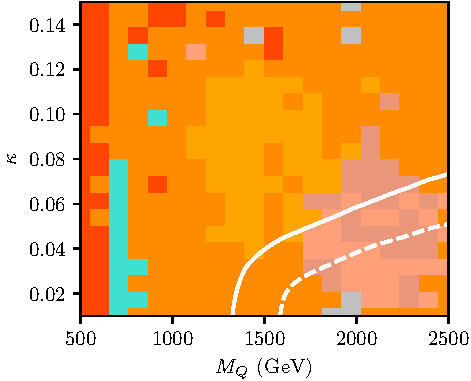
\includegraphics[width=0.45\textwidth]{Figures/VLQ/newm4l/1genWHZ001.pdf}\label{fig:BLpaper}}
  \subfloat[]{
    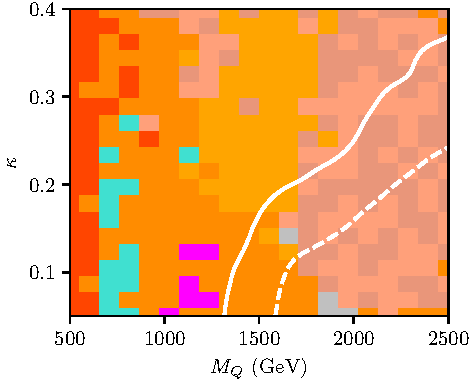
\includegraphics[width=0.45\textwidth]{Figures/VLQ/newm4l/2genWHZ001.pdf}\label{fig:BLcontur}} \\
  \vspace*{2ex}
  \begin{tabular}{llll}
        \swatch{navy}~ATLAS $\mu$+\MET{}+jet &
        \swatch{magenta}~ATLAS 4$\ell$ &
        \swatch{lightsalmon}~CMS $ee$+jet \\
        \swatch{darksalmon}~CMS $\mu\mu$+jet &
        \swatch{darkorange}~ATLAS $\mu\mu$+jet &
        \swatch{orangered}~ATLAS $ee$+jet \\
        \swatch{turquoise}~ATLAS $WW$ &
        \swatch{silver}~ATLAS jets &
        \swatch{cadetblue}~ATLAS $e$+\MET{}+jet & 
  \end{tabular}
  \vspace*{2ex}
  \caption{Dominant LHC analysis pools contributing to VLQ limit-setting in the $\kappa$ vs
    VLQ mass plane, where $\kappa$ is the coupling to third-generation SM quarks.
    All VLQ ($B, T, X, Y$) masses are set to be degenerate. The disfavoured regions
    are located above and to the left of the dashed (68\%~CL)
    and solid (95\%~CL) white contours respectively. The VLQ branching
    fraction to \WZH is~\WZHzoz. Plots are made with \contur 2.1.x and \rivet 3.1.4. %
  }
  \label{fig:vlq:newm4l}
\end{figure}